\chapter{Dynamická měření}\label{navesti:dynamickaMereni}
Dynamická měření přísunů radonu jsem provedl u tří objektů, viz tab.~\ref{tab:dynMer_prehled}.
\begin{table}[ht]
	\centering
	\caption{Objekty, v nichž jsem provedl dynamická měření. $dt$ značí dobu měření ve dnech (zaokrouhleno na celé dny včetně počátečního a posledního dne). V posledním sloupci je počet zón, na které byl daný objekt rozdělen.}
	\label{tab:dynMer_prehled}
	\begin{tabular}{lllll}
		\toprule
		Objekt & Rozsah měření & $dt$ [dny] & Typ objektu &$N$\\
		\midrule
		Skála 75, okr. Havlíčkův Brod & 23. 5. -- 5. 6. 2019 & 14 & chata & 3\\
		Hálková 980, Humpolec & 5. 6. -- 20. 6. 2019 & 15 & byt & 4\\
		Anglická 574, Dobřichovice & 9. 7. -- 30. 7. 2019 & 22 & rodinný dům & 3\\
		\bottomrule
	\end{tabular}
\end{table}

Vývoj OAR v čase v jednotlivých zónách byl měřen primárně TERA sondami~\cite{tera} a sekundárně měřiči radonu CANARY~\cite{canary}. CANARY měřáky byly použity jako záložní systém, tj. pokud by v některé zóně  TERA sonda selhala, pak by se OAR v této zóně brala z příslušného CANARY měřáku. %Zevrubné informace o těchto detektorech lze dohledat v kapitole~\ref{navesti:radon}.

Dále bylo potřeba měřit vývoj teploty, což je znalost nutná při vyhodnocování množství nasorbovaných indikačních plynů v TD detektorech a k určení hmotnostních koncentrací indikačních plynů  v zónách. K tomuto účelu byly použity dataloggery teploty a vlhkosti testo 174H~\cite{testo}. V případě objektu Hálková 980 byly k určení hmotnostních koncentrací použity teploty naměřené TERA sondami, jelikož v tomto objektu byl osazen pouze jeden datalogger testo 174H (jedná se jednopodlažní byt).

Do objektů byly při měřeních umístěny vždy jeden nebo dva zdroje radonu typu RF 2000 (viz podkapitola \ref{navesti:radon_zdroje}). U těchto zdrojů nás pro naše měření zajímají pouze radonové výdejnosti $W$, které představují definované absolutní přísuny radonu do zón, ve kterých jsou zdroje umístěny. Absolutními přísuny radonu je myšleno množství aktivity radonu, jenž se do zón dostane za hodinu, a tedy jejich jednotkou je \si{Bq/hod}. Radonové výdejnosti použitých zdrojů jsou uvedeny v tab.~\ref{tab:dynMer_zdroje}. Podělením $W$ objemem příslušné zóny můžeme dopočítat přísun radonu pocházející od daného zdroje do této zóny. 
\begin{table}[ht]
    \centering
    \caption{ID a radonové výdejnosti $W$ použitých radonových zdrojů typu RF 2000. Jako ID byla použita část výrobního čísla daného zdroje. Přebráno z certifikátů zdrojů, viz příloha~\ref{navesti:priloha_zdroje}.}
    \label{tab:dynMer_zdroje}
    \begin{tabular}{lr}
        \toprule
        ID & $W$ [\si{Bq/hod}]\\
        \midrule
        38 & 15588\\
        37 & 14436\\
        \bottomrule
    \end{tabular}
\end{table}

Před samotnými měřeními přísunů radonu v objektech bylo nejprve nutno provést srovnávací měření TERA sond, jelikož každá sonda má různou odezvu při stejné OAR. O tomto pojednává podkapitola~\ref{navesti:dynMer_TERA}. Další podkapitoly obsahují dynamická měření přísunů radonu v uvedených objektech. 

\section{TERA sondy}\label{navesti:dynMer_TERA}

Pro dynamická měření přísunů radonu mi byly poskytnuty čtyři TERA sondy s označením 8, 10, 88 a 112. Pro srovnání jejich odezev s reálnou hodnotou OAR byly vloženy do sudu (nádoba válcovitého tvaru) spolu s referenčním monitorem radonu AlphaGuard (ozn. AG)~\cite{alphaguard}. Hodnota OAR z AG byla brána jako reálná hodnota OAR. V obr.~\ref{fig:dynMer_sondySrovnani} jsou zobrazeny naměřené vývoje OAR v čase ze zkoumaných sond a z AG, v tab.~\ref{tab:dynMer_sondy} jsou k vidění nejdůležitější statistiky naměřených dat z každého monitoru.

\begin{figure}[H]
	\centering
	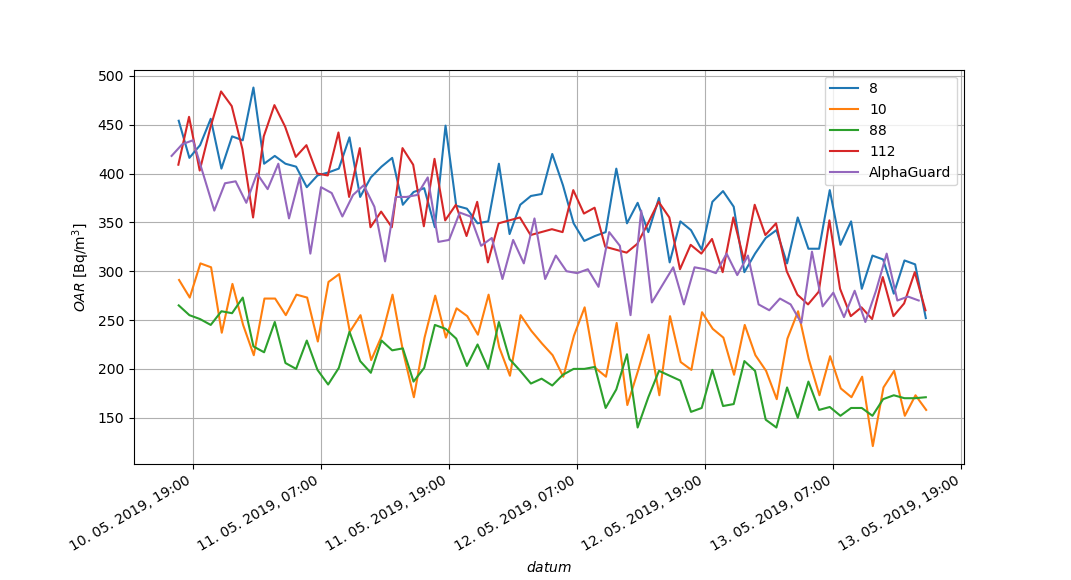
\includegraphics[width=1\linewidth]{images/sondy_srovnani}
	\caption{Vývoj OAR naměřený zkoumanými sondami a AG.}
	\label{fig:dynMer_sondySrovnani}
\end{figure}
\begin{table}[ht]
	\centering
	\caption{Statistiky vývojů OAR naměřených TERA sondami a AG v \si{Bq/m^3}.}
	\label{tab:dynMer_sondy}
	\begin{tabular}{lrrrrrrr}
		\toprule
		ID sondy &  count &  mean    &  min &  25\% &  50\% &  75\% &  max \\
		\midrule
		8          &     71 &   369  &  252 &  337 &  368 &  405 &  488 \\
		10         &     71 &   228  &  121 &  198 &  232 &  256 &  308 \\
		88         &     71 &   198  &  140 &  170 &  198 &  220 &  273 \\
		112        &     71 &   354  &  251 &  318 &  349 &  399 &  484 \\
		\midrule
		AG &     71 &   328  &  247 &  285 &  318 &  373 &  434 \\
		\bottomrule
	\end{tabular}
%&  std
      
%&   47
%&   41
%&   33
%&   58
      
%&   50
\end{table}

Pro opravu odezev byla zavedena pro každou sondu kalibrační konstanta $B$, která je definována následovně:
\begin{equation}
	B=\frac{OAR_A}{OAR_T}\,,
\end{equation}
kde $OAR_A$ je průměrná OAR z hodnot naměřených AG a $OAR_T$ je průměrná OAR z hodnot naměřených příslušnou TERA sondou. Pro získání věrohodné hodnoty koncentrace radonu z naměřené hodnoty danou sondou pak stačí tuto naměřenou hodnotu přenásobit $B$ náležející této sondě.

Relativní nejistoty kalibračních konstant byly odhadnuty na 10~\%. Určené kalibrační konstanty všech sond jsou k nahlédnutí v tab.~\ref{tab:dynMer_sondyB}. %Nejistoty kalibračních konstant určeny nebyly vzhledem k tomu, že se jedná o "veličinu", která se může při různých vnějších podmínkách měnit. Hlavním ovlivňujícím faktorem je velikost aerosolů v měřeném prostředí. Tato nespolehlivost TERA sond v poskytování věrohodných dat je dalším důvodem, proč byly použity měřáky radonu CANARY. Takto můžeme srovnávat data z více zdrojů.
%\begin{figure}[H]
	%\centering
	%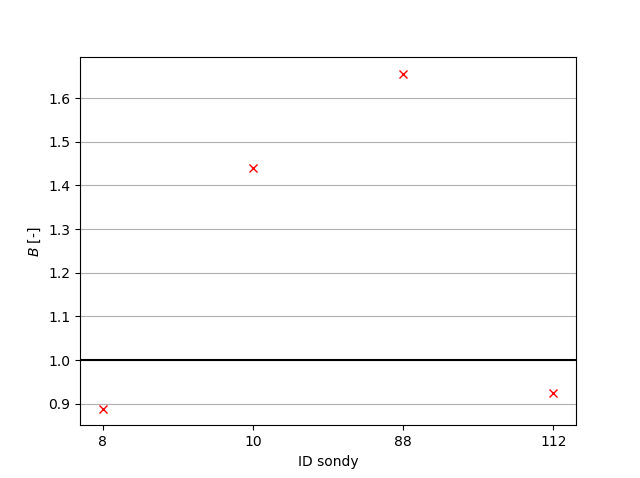
\includegraphics[width=0.7\linewidth]{images/sondy_B}
	%\caption{Kalibrační konstanty proměřených TERA sond. Černou čárou je vyznačen ideální případ, kdy se odezva sondy rovná skutečné OAR (resp. OAR naměřené AlphaGuardem).}
	%\label{fig:dynMer_sondyB}
%\end{figure}
\begin{table}[ht]
	\centering
	\caption{Kalibrační konstanty TERA sond odvozené od referenčního AG. Skutečná hodnota $OAR$ se vypočte ze vztahu $OAR=B\cdot OAR_T$, kde $OAR_T$ je naměřená obj. aktivita radonu danou TERA sondou. Nejistota kalibračních konstant byla odhadnuta na 10~\%.}
	\label{tab:dynMer_sondyB}
	\begin{tabular}{lr}
		\toprule
		ID sondy &     $B$ \\
		\midrule
		8   & 0,889$\pm$0,089\\
		10  & 1,440$\pm$0,140\\
		88  & 1,655$\pm$0,166\\
		112 & 0,925$\pm$0,093\\
		\bottomrule
	\end{tabular}
\end{table}
\section{Objekt Skála 75, okr. Havlíčkův Brod}
\subsection{Použitá měřidla}
\begin{itemize}
    \setlength\itemsep{0em}
	\item 14 vyvíječů (2x TMH, 2x TCE, 3x MDC, 3x MCH, 2x PCE, 2x PCH)
	\item 12 TD detektorů
	\item 4 CANARY monitory
	\item 4 TERA sondy
	\item 3 TESTO měřiče teploty a vlhkosti
	\item 2 zdroje radonu
\end{itemize}

\subsection{Naměřené OAR, objemy a teploty}

\begin{table}[H]
    \centering
    \caption{Objemy podlaží objektu, průměrné teploty naměřené v každém podlaží dataloggery testo 174H, odhadnuté atmosférické tlaky v každém podlaží a přiřazení číslování kompartmentů jednotlivým podlažím. Význam označení podlaží je vysvětlen v tab. \ref{tab:rovMer_podlazi}.}
    \label{tab:skala75_objemy}
    \begin{tabular}{lll}
\toprule
podlazi & $OAR$ [\si{Bq/m^3}] & $V$ [\si{m^3}] \\
\midrule
0 &           1094+/-55 &         40+/-8 \\
1 &            562+/-20 &        84+/-10 \\
2 &              51+/-2 &        97+/-15 \\
\bottomrule
\end{tabular}

\end{table}
\begin{figure}[H]
    \centering
    \includegraphics[width=1\textwidth]{skala75/OAR_dohromady.png}
    \caption{Vývoj OAR naměřený TERA sondami po aplikování kalibračních konstant (tab.~\ref{tab:dynMer_sondyB}). Pro další vyhodnocování byly OAR naměřené v přízemí v kuchyni a v ložnici zprůměrovány.}
    \label{fig:skala75_OARdohromady}
\end{figure}
\subsection{Objemové průtoky vzduchu}

\begin{table}[H]
    \centering
    \caption{Přehled použitých indikačních plynů a umístění jejich vyvíječů v objektu. V posledním sloupci jsou celkové odpary plynů ze všech jim odpovídajících vyvíječů.}
    \label{tab:skala75_indikacniPlyny}
    \begin{tabular}{lrrrr}
\toprule
ozn. & podlaží& odpar [mg] &    $M$ [g/mol] &    $U$ $\left[\si{\frac{ng}{ppm\cdot min}}\right]$\\
\midrule
TMH & 0 &192,50 &  450,0 &  8,000 \\
TCE & 0 &193,55 &  130,4 &  1,000 \\
MCH & 1 &472,27 &  350,0 &  8,000 \\
MDC & 1 &497,27 &  400,0 &  8,000 \\
PCH & 2 &230,88 &  450,0 &  8,000 \\
PCE & 2 & 96,54 &  165,8 &  1,385 \\
\bottomrule
\end{tabular}

\end{table}
\begin{table}[H]
    \centering
    \caption{Odezvy TD detektorů $R$ na všechny použité indikační plyny ve všech zónách.}
    \label{tab:skala75_odezvyTD}
    \begin{tabular}{lrr}
\toprule
plyn & zóna & $R$ [\si{ng}]               \\
\midrule
MCH & 1 & $  36,0\pm2,3$\\
    & 2 & $395,8\pm16,6$\\
    & 3 & $  50,8\pm2,3$\\
MDC & 1 & $  34,5\pm1,2$\\
    & 2 & $ 304,9\pm7,1$\\
    & 3 & $  47,2\pm1,2$\\
TMH & 1 & $145,3\pm26,0$\\
    & 2 & $  37,5\pm3,9$\\
    & 3 & $  20,2\pm2,4$\\
PCH & 1 & $  20,7\pm2,4$\\
    & 2 & $  26,9\pm0,7$\\
    & 3 & $ 182,2\pm4,6$\\
TCE & 1 & $191,8\pm14,5$\\
    & 2 & $  32,2\pm1,4$\\
    & 3 & $  25,0\pm1,2$\\
PCE & 1 & $     0,0\pm0,0$\\
    & 2 & $   2,6\pm0,1$\\
    & 3 & $ 136,9\pm4,1$\\
\bottomrule
\end{tabular}

\end{table}

\begin{table}[H]
    \centering
    \caption{Objemové průtoky vzduchu v \si{m^3/hod} pro všechny kombinace aplikovaných indikačních plynů. $n$ je výměna vzduchu vypočtená ze vztahu~\eqref{eq:prutoky_n}, $[n]=\si{1/hod}$.}
    \label{tab:skala75Prutoky_celkove}
%\begin{tabular}{l>{\raggedleft\arraybackslash}p{2.5cm}>{\raggedleft\arraybackslash}p{2.5cm}>{\raggedleft\arraybackslash}p{2.5cm}>{\raggedleft\arraybackslash}p{2.5cm}}
%\toprule
%{} & (TMH, MDC, PCE) & (TMH, MDC, PCH) & (TMH, MCH, PCE) & (TMH, MCH, PCH)\\ 
%\midrule
%$k_{12}$ & 4.139$\pm$1.044 & 3.771$\pm$0.994 & 3.445$\pm$0.874 & 3.128$\pm$0.830 \\          
%$k_{13}$ & 0.478$\pm$0.133 & 1.892$\pm$0.533 & 0.495$\pm$0.136 & 1.956$\pm$0.541 \\          
%$k_{21}$ & 0.656$\pm$0.152 & 0.574$\pm$0.137 & 0.525$\pm$0.126 & 0.455$\pm$0.114 \\          
%$k_{23}$ & 0.202$\pm$0.030 & 0.800$\pm$0.119 & 0.167$\pm$0.026 & 0.660$\pm$0.104 \\          
%$k_{31}$ &-0.019$\pm$0.005 & 0.854$\pm$0.233 &-0.015$\pm$0.004 & 0.881$\pm$0.237 \\          
%$k_{32}$ & 0.231$\pm$0.034 & 1.882$\pm$0.282 & 0.192$\pm$0.029 & 1.561$\pm$0.240 \\          
%$k_{1_E}$&12.492$\pm$2.813 &11.640$\pm$2.705 &13.100$\pm$2.886 &12.163$\pm$2.768 \\          
%$k_{2_E}$& 7.169$\pm$0.789 & 6.809$\pm$0.790 & 5.990$\pm$0.690 & 5.674$\pm$0.686 \\          
%$k_{3_E}$& 1.930$\pm$0.212 & 5.749$\pm$0.804 & 1.964$\pm$0.213 & 6.010$\pm$0.804 \\          
%$k_{1_I}$&16.471$\pm$3.007 &15.875$\pm$2.943 &16.530$\pm$3.022 &15.912$\pm$2.952 \\          
%$k_{2_I}$& 3.657$\pm$1.318 & 2.530$\pm$1.313 & 3.045$\pm$1.122 & 2.099$\pm$1.114 \\          
%$k_{3_I}$& 1.462$\pm$0.255 & 5.793$\pm$1.039 & 1.478$\pm$0.256 & 5.836$\pm$1.032 \\          
%\midrule
%$n$      & 0.091$\pm$0.014 & 0.102$\pm$0.015 & 0.089$\pm$0.014 & 0.101$\pm$0.015 \\
%\bottomrule
%\end{tabular}
%\vspace{0.5cm}

%\begin{tabular}{l>{\raggedleft\arraybackslash}p{2.5cm}>{\raggedleft\arraybackslash}p{2.5cm}>{\raggedleft\arraybackslash}p{2.5cm}>{\raggedleft\arraybackslash}p{2.5cm}}
    %\toprule
    %{} & (TCE, MDC, PCE) & (TCE, MDC, PCH) & (TCE, MCH, PCE) & (TCE, MCH, PCH) \\
    %\midrule
%$k_{12}$ & 3.330$\pm$0.551 & 2.965$\pm$0.519 & 2.774$\pm$0.468 & 2.462$\pm$0.438 \\
%$k_{13}$ & 0.462$\pm$0.081 & 1.828$\pm$0.322 & 0.476$\pm$0.082 & 1.879$\pm$0.326 \\
%$k_{21}$ & 0.215$\pm$0.034 & 0.188$\pm$0.032 & 0.172$\pm$0.030 & 0.149$\pm$0.028 \\
%$k_{23}$ & 0.203$\pm$0.029 & 0.802$\pm$0.118 & 0.168$\pm$0.026 & 0.662$\pm$0.104 \\
%$k_{31}$ &-0.006$\pm$0.001 & 0.279$\pm$0.060 &-0.005$\pm$0.001 & 0.288$\pm$0.061 \\
%$k_{32}$ & 0.230$\pm$0.034 & 1.922$\pm$0.283 & 0.191$\pm$0.029 & 1.595$\pm$0.241 \\
%$k_{1_E}$& 1.805$\pm$0.627 & 0.865$\pm$0.619 & 2.329$\pm$0.606 & 1.303$\pm$0.596 \\
%$k_{2_E}$& 7.579$\pm$0.796 & 7.166$\pm$0.798 & 6.322$\pm$0.699 & 5.960$\pm$0.695 \\
%$k_{3_E}$& 1.918$\pm$0.212 & 6.281$\pm$0.810 & 1.954$\pm$0.213 & 6.565$\pm$0.810 \\
%$k_{1_I}$& 5.388$\pm$0.840 & 5.191$\pm$0.872 & 5.412$\pm$0.771 & 5.207$\pm$0.812 \\
%$k_{2_I}$& 4.436$\pm$0.970 & 3.269$\pm$1.000 & 3.696$\pm$0.843 & 2.714$\pm$0.863 \\
%$k_{3_I}$& 1.478$\pm$0.231 & 5.852$\pm$0.926 & 1.497$\pm$0.232 & 5.908$\pm$0.914 \\
%\midrule                                                                           
%$n$      & 0.048$\pm$0.006 & 0.061$\pm$0.007 & 0.045$\pm$0.005 & 0.059$\pm$0.007 \\
%\bottomrule
%\end{tabular}
\begin{tabular}{l>{\raggedleft\arraybackslash}p{2.5cm}>{\raggedleft\arraybackslash}p{2.5cm}>{\raggedleft\arraybackslash}p{2.5cm}>{\raggedleft\arraybackslash}p{2.5cm}}
\toprule
{} & (TMH, MDC, PCE) & (TMH, MDC, PCH) & (TMH, MCH, PCE) & (TMH, MCH, PCH)\\ 
\midrule
$k_{12}$ &12,262$\pm$3,129 &  11,759$\pm$3,078 &  10,188$\pm$2,611 &   9,746$\pm$2,563 \\          
$k_{13}$ & 0,855$\pm$0,255 &   3,372$\pm$1,013 &   0,908$\pm$0,261 &   3,573$\pm$1,036 \\          
$k_{21}$ & 4,028$\pm$0,940 &   3,507$\pm$0,847 &   3,220$\pm$0,776 &   2,780$\pm$0,700 \\          
$k_{23}$ & 1,240$\pm$0,183 &   4,889$\pm$0,724 &   1,025$\pm$0,161 &   4,031$\pm$0,635 \\          
$k_{31}$ &-0,076$\pm$0,020 &   3,524$\pm$0,958 &  -0,061$\pm$0,016 &   3,611$\pm$0,968 \\          
$k_{32}$ & 0,931$\pm$0,137 &   5,967$\pm$0,967 &   0,774$\pm$0,117 &   4,945$\pm$0,820 \\          
&&&&\\
$k_{1_E}$&21,425$\pm$5,271 &  19,770$\pm$5,057 &  23,244$\pm$5,443 &  21,411$\pm$5,208 \\          
$k_{2_E}$&44,024$\pm$4,853 &  41,624$\pm$4,833 &  36,712$\pm$4,240 &  34,644$\pm$4,195 \\          
$k_{3_E}$& 7,712$\pm$0,849 &  24,294$\pm$3,199 &   7,850$\pm$0,853 &  25,127$\pm$3,209 \\          
$k_{1_I}$&30,590$\pm$6,206 &  27,869$\pm$6,140 &  31,181$\pm$6,093 &  28,339$\pm$6,017 \\          
$k_{2_I}$&36,099$\pm$5,855 &  32,294$\pm$5,917 &  29,994$\pm$5,043 &  26,764$\pm$5,073 \\          
$k_{3_I}$& 6,472$\pm$0,916 &  25,525$\pm$3,693 &   6,630$\pm$0,914 &  26,079$\pm$3,658 \\          
\midrule                                                                              
$n$      & 0,310$\pm$0,038 &   0,363$\pm$0,042 &   0,287$\pm$0,036 &   0,344$\pm$0,041 \\
\bottomrule
\end{tabular}
\vspace{0.5cm}

\begin{tabular}{l>{\raggedleft\arraybackslash}p{2.5cm}>{\raggedleft\arraybackslash}p{2.5cm}>{\raggedleft\arraybackslash}p{2.5cm}>{\raggedleft\arraybackslash}p{2.5cm}}
    \toprule
    {} & (TCE, MDC, PCE) & (TCE, MDC, PCH) & (TCE, MCH, PCE) & (TCE, MCH, PCH) \\
    \midrule
$k_{12}$ & 7,859$\pm$1,288 &   7,286$\pm$1,238 &   6,544$\pm$1,094 &   6,050$\pm$1,047 \\
$k_{13}$ & 0,893$\pm$0,159 &   3,523$\pm$0,631 &   0,927$\pm$0,162 &   3,647$\pm$0,641 \\
$k_{21}$ & 1,309$\pm$0,211 &   1,140$\pm$0,195 &   1,049$\pm$0,182 &   0,906$\pm$0,169 \\
$k_{23}$ & 1,235$\pm$0,180 &   4,874$\pm$0,715 &   1,023$\pm$0,159 &   4,025$\pm$0,628 \\
$k_{31}$ &-0,025$\pm$0,005 &   1,146$\pm$0,243 &  -0,020$\pm$0,004 &   1,176$\pm$0,245 \\
$k_{32}$ & 0,922$\pm$0,136 &   6,419$\pm$0,960 &   0,767$\pm$0,116 &   5,330$\pm$0,817 \\
&&&&\\
$k_{1_E}$& 2,474$\pm$1,325 &   0,539$\pm$1,320 &   3,713$\pm$1,256 &   1,616$\pm$1,248 \\
$k_{2_E}$&46,234$\pm$4,862 &  43,556$\pm$4,848 &  38,543$\pm$4,268 &  36,229$\pm$4,226 \\
$k_{3_E}$& 7,670$\pm$0,848 &  26,236$\pm$3,237 &   7,815$\pm$0,852 &  27,185$\pm$3,242 \\
$k_{1_I}$& 9,941$\pm$1,867 &   9,061$\pm$1,942 &  10,155$\pm$1,683 &   9,231$\pm$1,776 \\
$k_{2_I}$&39,997$\pm$5,039 &  35,866$\pm$5,149 &  33,303$\pm$4,414 &  29,780$\pm$4,477 \\
$k_{3_I}$& 6,439$\pm$0,891 &  25,404$\pm$3,517 &   6,613$\pm$0,889 &  26,019$\pm$3,470 \\
\midrule                                                                                 
$n$      & 0,239$\pm$0,028 &   0,298$\pm$0,034 &   0,212$\pm$0,025 &   0,275$\pm$0,031 \\
\bottomrule
\end{tabular}
\end{table}

\subsection{Přísuny radonu}
\begin{table}[H]
    \centering
    \caption{Přesně definované přísuny radonu ze zdrojů v \si{Bq/(m^3\cdot hod)}. Ve druhém sloupci je uvedeno, který zdroj byl umístěn v daném podlaží.}
    \label{tab:skala75_prisunyZdroj}
    \begin{tabular}{ll
        >{\collectcell\num}r<{\endcollectcell}
        @{${}\pm{}$}
        >{\collectcell\num}r<{\endcollectcell}}
        \toprule
        podlaží  &zdroj& \multicolumn{2}{r}{$Q_{zdroj}$}\\
        \midrule
        0 &38&400&51\\
        1 &37&114&13\\
        2 & NE &0&0\\
        \bottomrule
    \end{tabular}
\end{table}

\begin{table}[H]
    \centering
    \caption{Průměrné přísuny radonu v \si{Bq/(m^3\cdot hod)} souhrnně pro všechny kombinace indikačních plynů pro dynamické vyhodnocení.}
    \label{tab:skala75_prisunyDynamicky}
   \begin{tabular}{lrrrr}
\toprule
použité tracery & $Q_0$ $\left[\si{\frac{Bq}{m^3\cdot hod}}\right]$ & $Q_1$ $\left[\si{\frac{Bq}{m^3\cdot hod}}\right]$ & $Q_2$ $\left[\si{\frac{Bq}{m^3\cdot hod}}\right]$ & $Q_3$ $\left[\si{\frac{Bq}{m^3\cdot hod}}\right]$ \\
\midrule
(MDC, PCE, TCE, TMH) & 401+/-383 &    9+/-243 &       97+/-163 &                               -100+/-611 \\
(MDC, MCH, TCE, TMH) & 398+/-356 &   29+/-183 &      101+/-158 &                               -103+/-575 \\
\bottomrule
\end{tabular}

\end{table}
\subsubsection{Vyhodnocení v rovnovážném stavu}
\begin{table}[H]
    \centering
    \caption{Průměrné objemové koncentrace radonu naměřené TERA sondami umístěnými v uvedených podlažích. $\sigma_A$ je nejistota OAR typu A plynoucí ze statistického zpracování naměřených dat, $\sigma_B$ je nejistota OAR typu B plynoucí z ostatních zdrojů (statistika detekce, nejistota měřidla) a $\sigma$ je kombinovaná nejistota OAR. Při určování přísunů radonu v rovnovážném stavu byla použita pouze nejistota typu B, tj. $\sigma_B$. V posledním sloupci je průměrná citlivost TERA sond vypočtená z naměřených dat (tj. z naměřeného počtu impulzů a naměřeného OAR). Tato citlivost byla použita pro výpočet $\sigma_B$.}
    \label{tab:skala75_OARprumerne}
    \begin{tabular}{llrrrrr}
\toprule
ID sondy&podlaží& OAR [\si{Bq/m^3}]& $\sigma_A$ & $\sigma_B$ &$\sigma$& $\overline{c}$ $\left[\si{\frac{imp}{hod}/\frac{Bq}{m^3}}\right]$\\ 
\midrule
8  &0 & 458 & 309 & 33 & 311&0,405\\
10 &1 & 789 & 485 & 43 & 487&0,433\\
112&1 & 633 & 282 & 37 & 284&0,464\\
88 &2 & 276 & 356 & 31 & 358&0,296\\
\bottomrule
    \end{tabular}
\end{table}

\begin{table}[H]
    \centering
    \caption{Průměrné OAR naměřené CANARY měřáky umístěnými v daných podlažích.}
    \label{tab:skala75_OARprumerne_CANARY}
    \begin{tabular}{llr
        %>{\collectcell\num}r<{\endcollectcell}
        %@{${}\pm{}$}
        %>{\collectcell\num}r<{\endcollectcell}
        }
        \toprule
        ID měřáku & podlaží & OAR [\si{Bq/m^3}]\\
        \midrule
        1 & 0 & $381\pm38$\\
        2 & 1 & $419\pm42$\\
        4 & 1 & $465\pm47$\\
        3 & 2 & $156\pm16$\\
        \bottomrule
    \end{tabular}
\end{table}

\begin{table}[H]
    \centering
    \caption{Přísuny radonu určené z průměrných hodnot vývojů OAR naměřených TERA sondami. Jednotkou přísunů radonu je \si{Bq/(m^3\cdot hod)}.}
    \label{tab:skala75_prisunyRovnovazne}
   \begin{tabular}{llll}
\toprule
{} & $Q_0$ $\left[\si{\frac{Bq}{m^3\cdot hod}}\right]$ & $Q_1$ $\left[\si{\frac{Bq}{m^3\cdot hod}}\right]$ & $Q_2$ $\left[\si{\frac{Bq}{m^3\cdot hod}}\right]$ \\
\midrule
(TMH, MDC, PCE) &                                          335+/-90 &                                          236+/-42 &                                            18+/-6 \\
(TMH, MDC, PCH) &                                          323+/-88 &                                          231+/-42 &                                           63+/-24 \\
(TMH, MCH, PCE) &                                          347+/-89 &                                          197+/-36 &                                            19+/-6 \\
(TMH, MCH, PCH) &                                          334+/-87 &                                          192+/-35 &                                           70+/-24 \\
(TCE, MDC, PCE) &                                          111+/-28 &                                          249+/-41 &                                            17+/-6 \\
(TCE, MDC, PCH) &                                          108+/-28 &                                          243+/-41 &                                           62+/-23 \\
(TCE, MCH, PCE) &                                          115+/-26 &                                          208+/-35 &                                            19+/-6 \\
(TCE, MCH, PCH) &                                          111+/-27 &                                          203+/-35 &                                           70+/-23 \\
\bottomrule
\end{tabular}

\end{table}

\begin{table}[H]
    \centering
    \caption{Přísuny radonu určené z průměrných hodnot vývojů OAR naměřených CANARY měřáky. Jednotkou přísunů radonu je \si{Bq/(m^3\cdot hod)}.}
    \label{tab:skala75_prisunyRovnovazneCANARY}
   \begin{tabular}{lllll}
\toprule
{} & $Q_1$ $\left[\si{\frac{Bq}{m^3\cdot hod}}\right]$ & $Q_2$ $\left[\si{\frac{Bq}{m^3\cdot hod}}\right]$ & $Q_3$ $\left[\si{\frac{Bq}{m^3\cdot hod}}\right]$ & $Q_4$ $\left[\si{\frac{Bq}{m^3\cdot hod}}\right]$ \\
\midrule
(MDC, PCE, TCE, TMH) &                                         200+/-168 &                                         139+/-356 &                                          75+/-127 &                                         165+/-172 \\
(MDC, MCH, TCE, TMH) &                                          201+/-78 &                                          141+/-75 &                                           76+/-59 &                                          166+/-80 \\
\bottomrule
\end{tabular}

\end{table}
%\subsection{Přeurčená varianta}

%\begin{table}[H]
    %\centering
    %\caption{Průtoky vzduchu mezi jednotlivými zónami. Vnější prostředí je označeno číslem 4.}
    %\label{tab:skala75Preurcena_prutoky}
    %\begin{tabular}{ll}
\toprule
k12 &  3.0+/-1.9 \\
k13 &  0.7+/-1.9 \\
k21 &  0.2+/-0.7 \\
k23 &  0.3+/-0.7 \\
k31 &  0.1+/-1.3 \\
k32 &  0.6+/-1.3 \\
k14 &  2.9+/-3.3 \\
k24 &  6.9+/-1.3 \\
k34 &  3.1+/-2.2 \\
k41 &      6+/-5 \\
k42 &  3.7+/-2.9 \\
k43 &      3+/-4 \\
\bottomrule
\end{tabular}

%\end{table}
%\begin{table}[H]
    %\centering
    %\caption{Statistiky vypočítaných přísunů radonu $Q$ do jednotlivých zón.}
    %\label{tab:skala75Preurcena_objemy}
    %\begin{tabular}{lrrr}
\toprule
{} &  $Q_0$ $\left[\si{\frac{Bq}{m^3\cdot hod}}\right]$ &  $Q_1$ $\left[\si{\frac{Bq}{m^3\cdot hod}}\right]$ &  $Q_2$ $\left[\si{\frac{Bq}{m^3\cdot hod}}\right]$ \\
\midrule
count &                                                309 &                                                309 &                                                309 \\
mean  &                                                 70 &                                                 34 &                                                 10 \\
std   &                                                134 &                                                156 &                                                101 \\
min   &                                               -991 &                                               -419 &                                               -305 \\
25\\%   &                                                 18 &                                                -14 &                                                -20 \\
50\\%   &                                                 52 &                                                 27 &                                                 -0 \\
75\\%   &                                                109 &                                                 86 &                                                 22 \\
max   &                                                879 &                                               2169 &                                                914 \\
\bottomrule
\end{tabular}

%\end{table}

%\begin{figure}[H]
    %\centering
    %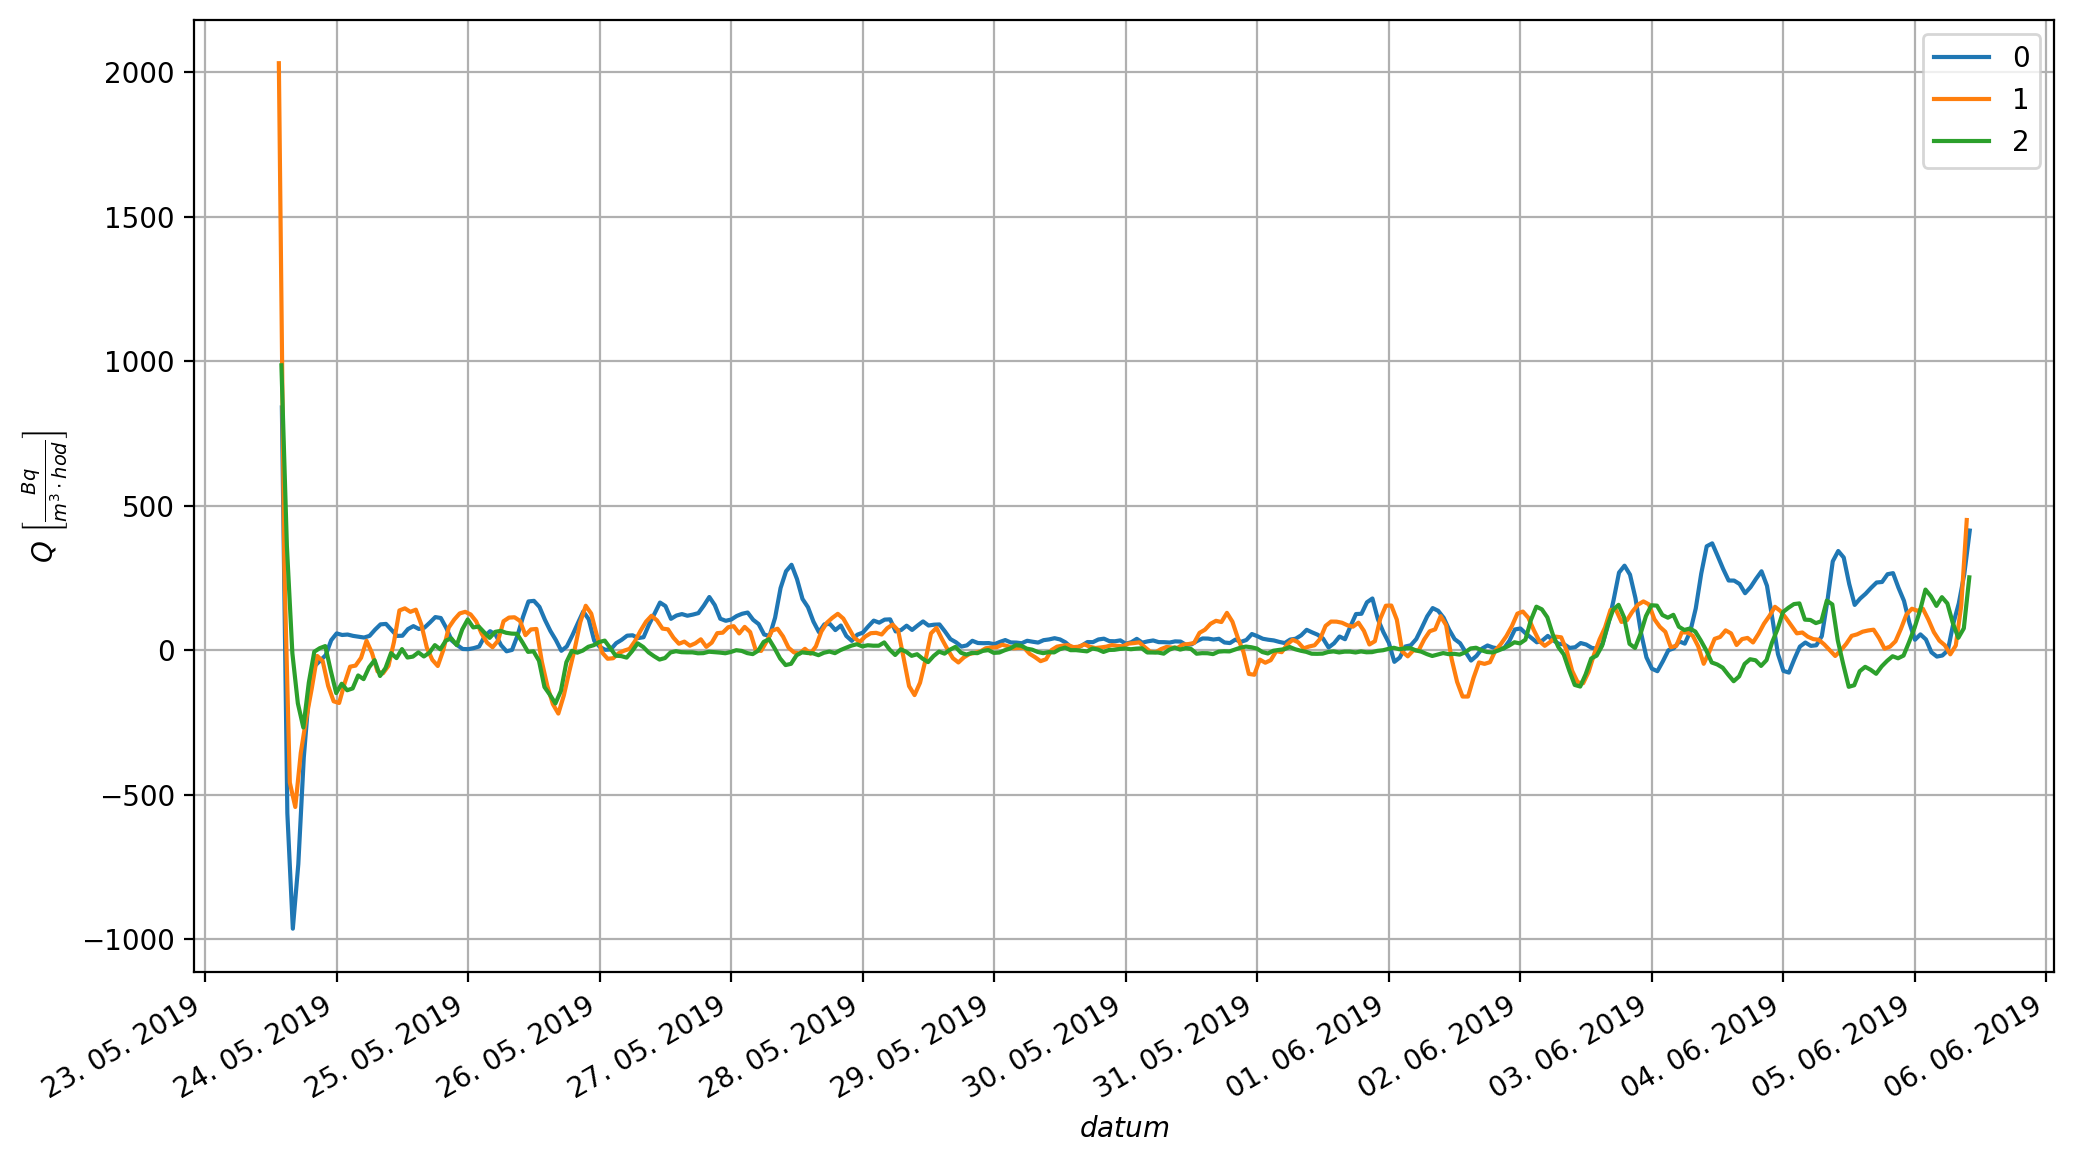
\includegraphics[width=\textwidth]{skala75/prisuny_preurcena.png}
    %\caption{Přísuny radonu. Popisky v legendě značí podlaží.}
    %\label{fig:skala75Preurcena_prisuny}
%\end{figure}

\section{Objekt Hálková 980, Humpolec}
\subsection{Použitá měřidla}
\begin{itemize}
    \setlength\itemsep{0em}
	\item 20 vyvíječů (4x MDC, 4x MCH, 4x PCE, 4x TCE, 4x TMH)
	\item 8 TD detektorů
	\item 4 CANARY monitory
	\item 4 TERA sondy
	\item 3 TESTO měřiče teploty a vlhkosti
	\item 1 zdroj radonu
\end{itemize}

\subsection{Naměřené OAR, objemy a teploty}

\begin{table}[H]
    \centering
    \caption{Přiřazení číslování kompartmentů jednotlivým podlažím, objemy všech zón objektu, průměrné teploty naměřené v každém zóně TERA sondami, odhadnuté atmosférické tlaky v každém zóně a průměrné OAR naměřené TERA sondami ($OAR_T$) a CANARY měřáky ($OAR_C$). OAR jsou uvedené v \si{Bq/m^3}.}
    \label{tab:halkova980_objemy}
    \begin{tabular}{lll}
\toprule
podlazi & $OAR$ [\si{Bq/m^3}] & $V$ [\si{m^3}] \\
\midrule
0 &           1094+/-55 &         40+/-8 \\
1 &            562+/-20 &        84+/-10 \\
2 &              51+/-2 &        97+/-15 \\
\bottomrule
\end{tabular}

\end{table}
\begin{figure}[H]
    \centering
    \includegraphics[width=1\textwidth]{halkova980/OAR_dohromady.png}
    \caption{Vývoj OAR naměřený TERA sondami po aplikování kalibračních konstant (tab.~\ref{tab:dynMer_sondyB}).}
    \label{fig:halkova980_OARdohromady}
\end{figure}

\subsection{Objemové průtoky vzduchu}

\begin{table}[H]
    \centering
    \caption{Přehled použitých indikačních plynů a umístění jejich vyvíječů v objektu. V posledním sloupci jsou celkové odpary plynů ze všech jim odpovídajících vyvíječů.}
    \label{tab:halkova980_indikacniPlyny}
    \begin{tabular}{lrrrr}
\toprule
ozn. & podlaží& odpar [mg] &    $M$ [g/mol] &    $U$ $\left[\si{\frac{ng}{ppm\cdot min}}\right]$\\
\midrule
TMH & 0 &192,50 &  450,0 &  8,000 \\
TCE & 0 &193,55 &  130,4 &  1,000 \\
MCH & 1 &472,27 &  350,0 &  8,000 \\
MDC & 1 &497,27 &  400,0 &  8,000 \\
PCH & 2 &230,88 &  450,0 &  8,000 \\
PCE & 2 & 96,54 &  165,8 &  1,385 \\
\bottomrule
\end{tabular}

\end{table}
\begin{table}[H]
    \centering
    \caption{Odezvy TD detektorů $R$ na všechny použité indikační plyny ve všech zónách.}
    \label{tab:halkova980_odezvyTD}
    \begin{tabular}{lrr}
\toprule
plyn & zóna & $R$ [\si{ng}]               \\
\midrule
MCH & 1 & $  36,0\pm2,3$\\
    & 2 & $395,8\pm16,6$\\
    & 3 & $  50,8\pm2,3$\\
MDC & 1 & $  34,5\pm1,2$\\
    & 2 & $ 304,9\pm7,1$\\
    & 3 & $  47,2\pm1,2$\\
TMH & 1 & $145,3\pm26,0$\\
    & 2 & $  37,5\pm3,9$\\
    & 3 & $  20,2\pm2,4$\\
PCH & 1 & $  20,7\pm2,4$\\
    & 2 & $  26,9\pm0,7$\\
    & 3 & $ 182,2\pm4,6$\\
TCE & 1 & $191,8\pm14,5$\\
    & 2 & $  32,2\pm1,4$\\
    & 3 & $  25,0\pm1,2$\\
PCE & 1 & $     0,0\pm0,0$\\
    & 2 & $   2,6\pm0,1$\\
    & 3 & $ 136,9\pm4,1$\\
\bottomrule
\end{tabular}

\end{table}

\begin{table}[H]
    \centering
    \caption{Objemové průtoky vzduchu mezi zónami v \si{m^3/hod} a výměna vzduchu $n$ v \si{hod^{-1}}.}
    \label{tab:halkova980_prutoky}
    \begin{tabular}{l
        >{\collectcell\num}r<{\endcollectcell}
        @{${}\pm{}$}
        >{\collectcell\num}r<{\endcollectcell}
        >{\collectcell\num}r<{\endcollectcell}
        @{${}\pm{}$}
        >{\collectcell\num}r<{\endcollectcell}
}
%\begin{tabular}{l>{\raggedleft\arraybackslash}p{2.5cm}>{\raggedleft\arraybackslash}p{2.5cm}}
\toprule
%{} & (MDC, PCE, TCE, TMH) & (MDC, MCH, TCE, TMH) \\
{} & \multicolumn{2}{r}{(MDC, PCE,} & \multicolumn{2}{r}{(MDC, MCH,} \\
{} & \multicolumn{2}{r}{TCE, TMH)} &   \multicolumn{2}{r}{TCE, TMH)} \\
\midrule
$k_{12}$          &    12,2&4,9 &          40,4&13,4   \\
$k_{13}$          &     4,8&8,9 &           11,9&8,2   \\
$k_{14}$          &   96,0&35,9 &          92,9&34,0   \\
$k_{21}$          &   31,3&27,5 &          40,5&14,8   \\
$k_{23}$          &    17,9&7,9 &            4,4&3,3   \\
$k_{24}$          &   13,8&24,1 &          19,7&12,7   \\
$k_{31}$          &   63,4&26,0 &          62,6&26,1   \\
$k_{32}$          &     1,9&2,8 &            6,2&8,9   \\
$k_{34}$          &   46,9&24,3 &          46,5&23,9   \\
$k_{41}$          &   76,3&37,1 &          74,6&37,7   \\
$k_{42}$          &     4,1&4,1 &          13,6&13,2   \\
$k_{43}$          &    18,0&9,7 &           20,4&9,9   \\
&\multicolumn{2}{r}{}&\multicolumn{2}{r}{}\\
$k_{1_E}$          &   72,6&18,6 &          45,3&11,8   \\
$k_{2_E}$          &  -39,9&15,3 &           12,1&4,6   \\
$k_{3_E}$          &  -27,3&12,3 &          -31,5&8,8   \\
$k_{4_E}$          &   50,9&18,7 &          41,7&13,4   \\
$k_{1_I}$          &   14,7&67,4 &          12,7&62,2   \\
$k_{2_I}$          &    5,0&41,0 &          16,6&29,1   \\
$k_{3_I}$          &   44,2&40,8 &          47,1&39,8   \\
$k_{4_I}$          &   -7,5&65,6 &          -8,8&61,4   \\
\midrule
$n$  &     0,4&0,2 &            0,4&0,1   \\   
\bottomrule
\end{tabular}

    
    
    
    
    
    
    
    
    
    
    
    
    
    
    
    
    
    
    
    
    


\end{table}

\subsection{Přísuny radonu}

\begin{table}[H]
    \centering
    \caption{Přesně definované přísuny radonu ze zdrojů v \si{Bq/(m^3\cdot hod)}. Ve druhém sloupci je uvedeno, který zdroj byl umístěn v dané zóně.}
    \label{tab:halkova980_prisunyZdroj}
    \begin{tabular}{ll
        >{\collectcell\num}r<{\endcollectcell}
        @{${}\pm{}$}
        >{\collectcell\num}r<{\endcollectcell}
    }
        \toprule
        zóna &zdroj  & \multicolumn{2}{r}{$Q_{zdroj}$}\\
        \midrule
        1 &38& 332&64\\
        2 &NE    & 0&0   \\
        3 &NE    & 0&0   \\
        4 &NE    & 0&0   \\
        \bottomrule
    \end{tabular}
\end{table}
%\begin{table}[H]
    %\centering
    %\caption{Statistiky vypočítaných přísunů radonu $Q$ do jednotlivých podlaží.}
    %\label{tab:halkova980_prisuny}
    %\begin{tabular}{lrrr}
\toprule
{} &  $Q_0$ $\left[\si{\frac{Bq}{m^3\cdot hod}}\right]$ &  $Q_1$ $\left[\si{\frac{Bq}{m^3\cdot hod}}\right]$ &  $Q_2$ $\left[\si{\frac{Bq}{m^3\cdot hod}}\right]$ \\
\midrule
count &                                                284 &                                                284 &                                                284 \\
mean  &  3035 &      4367 &     677 \\
std   &  2122 &      2579 &    1470 \\
min   &                                                652 &                                                319 &                                               -934 \\
25%   &                                               1377 &                                               2000 &                                               -224 \\
50%   &                                               2397 &                                               4104 &                                                 11 \\
75%   &                                               3830 &                                               6310 &                                               1389 \\
max   &                                               9130 &                                               9673 &                                               4902 \\
\bottomrule
\end{tabular}

%\end{table}
\begin{table}[H]
    \centering
    \caption{Průměrné přísuny radonu do zón (ne podlaží!) pro všechny možné kombinace indikačních plynů za použití průměrných hodnot vývojů OAR naměřených TERA sondami (rovnovážné vyhodnocení).}
    \label{tab:halkova980_prisunyRovnovazne}
    \begin{tabular}{llll}
\toprule
{} & $Q_0$ $\left[\si{\frac{Bq}{m^3\cdot hod}}\right]$ & $Q_1$ $\left[\si{\frac{Bq}{m^3\cdot hod}}\right]$ & $Q_2$ $\left[\si{\frac{Bq}{m^3\cdot hod}}\right]$ \\
\midrule
(TMH, MDC, PCE) &                                          335+/-90 &                                          236+/-42 &                                            18+/-6 \\
(TMH, MDC, PCH) &                                          323+/-88 &                                          231+/-42 &                                           63+/-24 \\
(TMH, MCH, PCE) &                                          347+/-89 &                                          197+/-36 &                                            19+/-6 \\
(TMH, MCH, PCH) &                                          334+/-87 &                                          192+/-35 &                                           70+/-24 \\
(TCE, MDC, PCE) &                                          111+/-28 &                                          249+/-41 &                                            17+/-6 \\
(TCE, MDC, PCH) &                                          108+/-28 &                                          243+/-41 &                                           62+/-23 \\
(TCE, MCH, PCE) &                                          115+/-26 &                                          208+/-35 &                                            19+/-6 \\
(TCE, MCH, PCH) &                                          111+/-27 &                                          203+/-35 &                                           70+/-23 \\
\bottomrule
\end{tabular}

\end{table}

\begin{table}[H]
    \centering
    \caption{Průměrné přísuny radonu do zón pro všechny možné kombinace indikačních plynů vypočtené z průměrných hodnot vývojů OAR naměřených CANARY měřáky.}
    \label{tab:halkova980_prisunyRovnovazneCANARY}
    \begin{tabular}{lllll}
\toprule
{} & $Q_1$ $\left[\si{\frac{Bq}{m^3\cdot hod}}\right]$ & $Q_2$ $\left[\si{\frac{Bq}{m^3\cdot hod}}\right]$ & $Q_3$ $\left[\si{\frac{Bq}{m^3\cdot hod}}\right]$ & $Q_4$ $\left[\si{\frac{Bq}{m^3\cdot hod}}\right]$ \\
\midrule
(MDC, PCE, TCE, TMH) &                                         200+/-168 &                                         139+/-356 &                                          75+/-127 &                                         165+/-172 \\
(MDC, MCH, TCE, TMH) &                                          201+/-78 &                                          141+/-75 &                                           76+/-59 &                                          166+/-80 \\
\bottomrule
\end{tabular}

\end{table}

\subsection{Zpětné ověření}

\subsubsection{OAR}
\begin{table}[H]
    \centering
    \caption{Průměrné OAR ve všech podlažích vypočítané pomocí rovnice~\eqref{eq:maticovy_zapis_rovnovaha} za použití průtoků vzduchu z tab.~\ref{tab:halkova980_prutoky} a přísunů radonu pocházejících od zdrojů RF 2000 (tab.~\ref{tab:halkova980_prisunyZdroj}) a průměrné OAR naměřené CANARY měřáky.}
    \label{tab:halkova980_OAR_zpetne}
    \begin{tabular}{lrrrr}
        \toprule
        & $a_1$ [\si{Bq/m^3}] &  $a_2$ [\si{Bq/m^3}]& $a_3$ [\si{Bq/m^3}]& $a_4$ [\si{Bq/m^3}]\\
        \midrule
(MDC, PCE, TCE, TMH) & $200\pm168$          &$139\pm356$     &$75\pm127$       &$165\pm172$ \\
(MDC, MCH, TCE, TMH) & $201\pm\ \,78$       &$ 141\pm\ \,75$ &$76\pm\ \,59$    &$ 166\pm\ \,80$ \\
\midrule
       naměřené      & $210\pm\ \,21$       & $97\pm\ \,10$  &$72\pm\ \,\ \,7$ &$139\pm\ \,14$\\
        \bottomrule
    \end{tabular}
\end{table}

\section{Objekt Anglická 574, Dobřichovice}

\subsection{Použitá měřidla}
\begin{itemize}
    \setlength\itemsep{0em}
	\item 12 vyvíječů (4x MCH, 4x MDC, 4x PCH)
	\item 12 TD detektorů
	\item 2 blank TD detektory 
	\item 4 CANARY monitory
	\item 4 TERA sondy
	\item 3 TESTO měřiče teploty a vlhkosti
	\item 2 zdroje radonu
\end{itemize}

\subsection{Naměřené OAR, objemy a teploty}

\begin{table}[H]
    \centering
    \caption{Objemy všech podlaží objektu, průměrné teploty naměřené v každém podlaží TERA sondami, odhadnuté atmosférické tlaky v každém podlaží, průměrné OAR naměřené TERA sondami ($OAR_T$) a CANARY měřáky ($OAR_C$) a přiřazení číslování kompartmentů jednotlivým podlažím. OAR jsou uvedené v \si{Bq/m^3}.}
    \label{tab:anglicka574_objemy}
    \begin{tabular}{lll}
\toprule
podlazi & $OAR$ [\si{Bq/m^3}] & $V$ [\si{m^3}] \\
\midrule
0 &           1094+/-55 &         40+/-8 \\
1 &            562+/-20 &        84+/-10 \\
2 &              51+/-2 &        97+/-15 \\
\bottomrule
\end{tabular}

\end{table}
\begin{figure}[H]
    \centering
    \includegraphics[width=1\textwidth]{anglicka574/OAR_dohromady.png}
    \caption{Vývoj OAR naměřený TERA sondami po aplikování kalibračních konstant (tab.~\ref{tab:dynMer_sondyB}).}
    \label{fig:anglicka574_OARdohromady}
\end{figure}

\subsection{Objemové průtoky vzduchu}

\begin{table}[H]
    \centering
    \caption{Přehled použitých indikačních plynů a umístění jejich vyvíječů v objektu. V posledním sloupci jsou celkové odpary plynů ze všech jim odpovídajících vyvíječů.}
    \label{tab:anglicka574_indikacniPlyny}
    \begin{tabular}{lrrrr}
\toprule
ozn. & podlaží& odpar [mg] &    $M$ [g/mol] &    $U$ $\left[\si{\frac{ng}{ppm\cdot min}}\right]$\\
\midrule
TMH & 0 &192,50 &  450,0 &  8,000 \\
TCE & 0 &193,55 &  130,4 &  1,000 \\
MCH & 1 &472,27 &  350,0 &  8,000 \\
MDC & 1 &497,27 &  400,0 &  8,000 \\
PCH & 2 &230,88 &  450,0 &  8,000 \\
PCE & 2 & 96,54 &  165,8 &  1,385 \\
\bottomrule
\end{tabular}

\end{table}
\begin{table}[H]
    \centering
    \caption{Odezvy TD detektorů $R$ na všechny použité indikační plyny ve všech zónách.}
    \label{tab:anglicka574_odezvyTD}
    \begin{tabular}{lrr}
\toprule
plyn & zóna & $R$ [\si{ng}]               \\
\midrule
MCH & 1 & $  36,0\pm2,3$\\
    & 2 & $395,8\pm16,6$\\
    & 3 & $  50,8\pm2,3$\\
MDC & 1 & $  34,5\pm1,2$\\
    & 2 & $ 304,9\pm7,1$\\
    & 3 & $  47,2\pm1,2$\\
TMH & 1 & $145,3\pm26,0$\\
    & 2 & $  37,5\pm3,9$\\
    & 3 & $  20,2\pm2,4$\\
PCH & 1 & $  20,7\pm2,4$\\
    & 2 & $  26,9\pm0,7$\\
    & 3 & $ 182,2\pm4,6$\\
TCE & 1 & $191,8\pm14,5$\\
    & 2 & $  32,2\pm1,4$\\
    & 3 & $  25,0\pm1,2$\\
PCE & 1 & $     0,0\pm0,0$\\
    & 2 & $   2,6\pm0,1$\\
    & 3 & $ 136,9\pm4,1$\\
\bottomrule
\end{tabular}

\end{table}

\begin{table}[H]
    \centering
    \caption{Objemové průtoky vzduchu mezi zónami v \si{m^3/hod} a výměna vzduchu $n$ v \si{hod^{-1}}.}
    \label{tab:anglicka574_prutoky}
    \begin{tabular}{lllll}
\toprule
{} &            0 &          1 &              2 & vnější prostředí \\
\midrule
0                &            0 &  1.3+/-0.4 &  0.033+/-0.029 &           45+/-8 \\
1                &    2.5+/-0.7 &          0 &    0.47+/-0.16 &           23+/-4 \\
2                &  0.14+/-0.12 &  1.3+/-0.4 &              0 &       16.2+/-2.9 \\
vnější prostředí &       44+/-8 &     23+/-4 &     17.1+/-2.9 &                0 \\
\bottomrule
\end{tabular}

\end{table}
\subsection{Přísuny radonu}

\begin{table}[H]
    \centering
    \caption{Přesně definované přísuny radonu ze zdrojů v \si{Bq/(m^3\cdot hod)}. Ve druhém sloupci je uvedeno, ve kterém podlaží byly zdroje umístěny.}
    \label{tab:anglicka574_prisunyZdroj}
    \begin{tabular}{ll
        >{\collectcell\num}r<{\endcollectcell}
        @{${}\pm{}$}
        >{\collectcell\num}r<{\endcollectcell}}
        \toprule
        podlaží  &zdroj& \multicolumn{2}{r}{$Q_{zdroj}$}\\
        \midrule
        0 &38 \& 37&455&90\\
        1 & NE &0&0\\
        2 & NE &0&0\\
        \bottomrule
    \end{tabular}
\end{table}

\begin{figure}[ht]
    \begin{subfigure}{\textwidth}
        \centering
        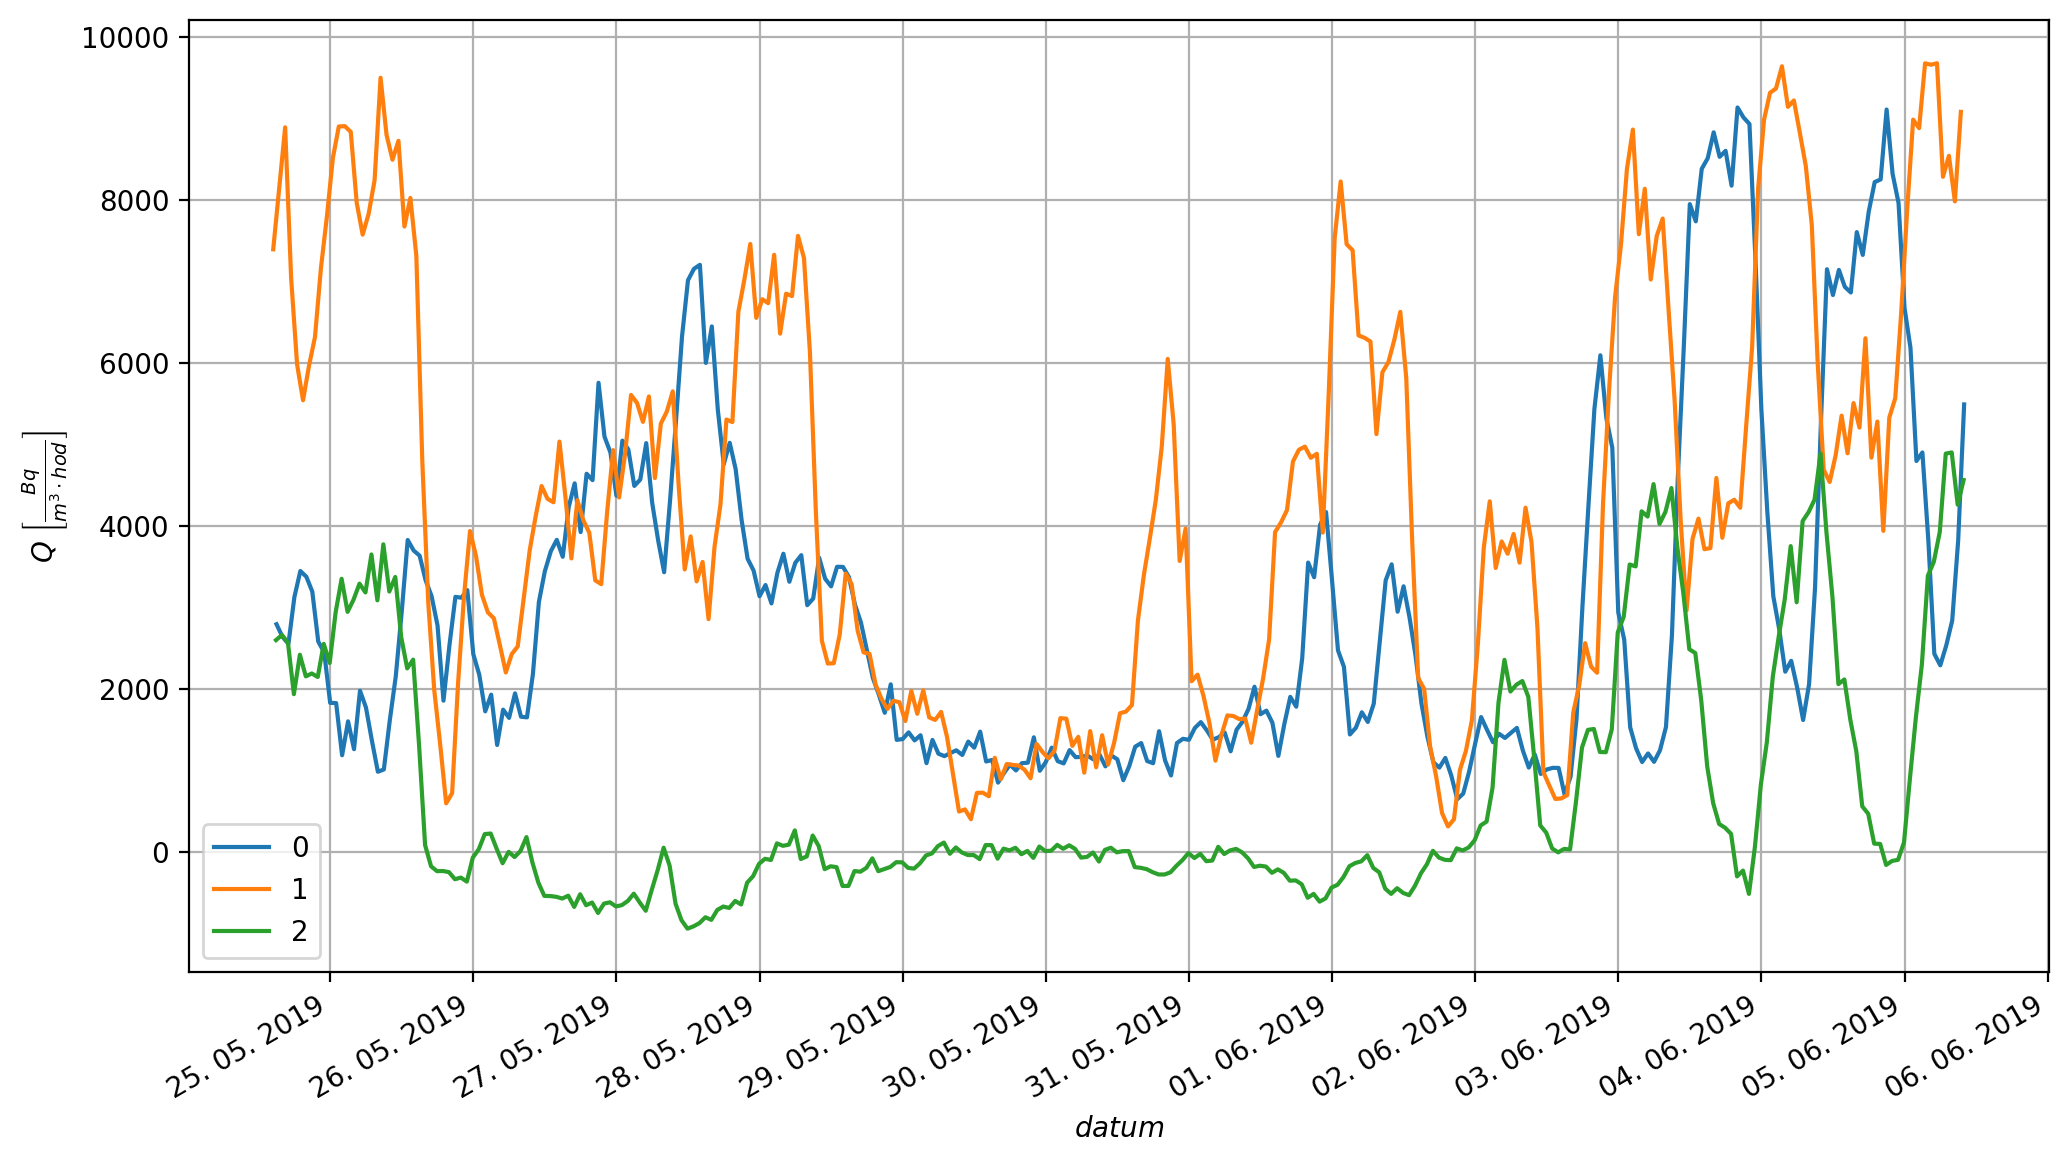
\includegraphics[width=\textwidth]{anglicka574/prisuny.png}
        \caption{}
        \label{fig:anglicka574_prisuny}
    \end{subfigure}
    \begin{subfigure}{\textwidth}
        \centering
        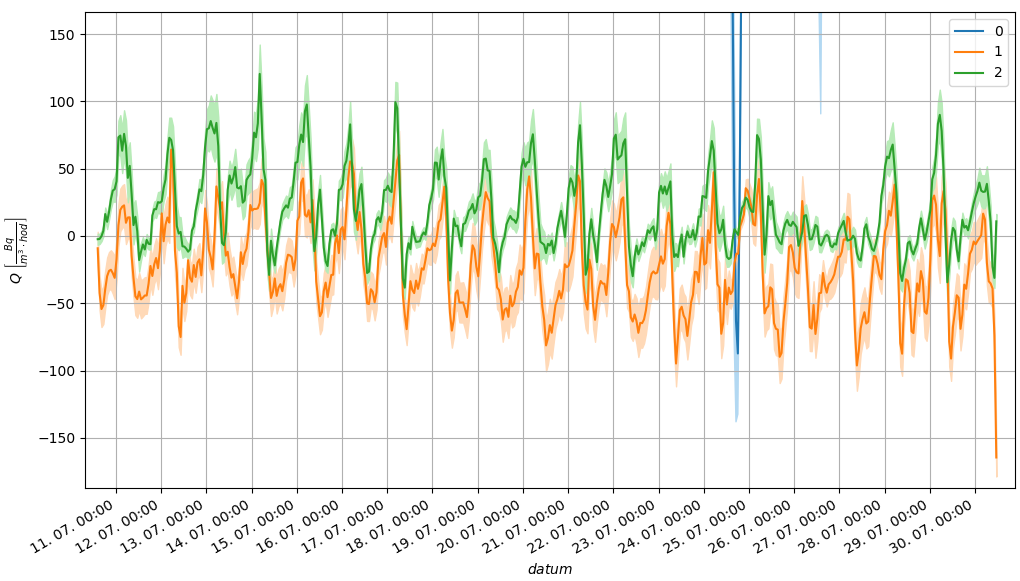
\includegraphics[width=\textwidth]{anglicka574/prisuny_zoom.png}
        \caption{}
        \label{fig:anglicka574_prisunyZoom}
    \end{subfigure}
    \caption{V (a) jsou určené časové vývoje přísunů radonu do jednotlivých podlaží. V (b) jsou přiblížené přísuny radonu do přízemí a prvního patra. Oblasti označené zesvětlenou barvou značí nejistotu přísunů radonu při faktoru pokrytí $k=1$.}
\end{figure}
\begin{table}[H]
    \centering
    \caption{Statistiky vypočítaných přísunů radonu $Q$ do jednotlivých podlaží.}
    \label{tab:anglicka574_prisuny}
    \begin{tabular}{lrrr}
\toprule
{} &  $Q_0$ $\left[\si{\frac{Bq}{m^3\cdot hod}}\right]$ &  $Q_1$ $\left[\si{\frac{Bq}{m^3\cdot hod}}\right]$ &  $Q_2$ $\left[\si{\frac{Bq}{m^3\cdot hod}}\right]$ \\
\midrule
count &                                                284 &                                                284 &                                                284 \\
mean  &  3035 &      4367 &     677 \\
std   &  2122 &      2579 &    1470 \\
min   &                                                652 &                                                319 &                                               -934 \\
25%   &                                               1377 &                                               2000 &                                               -224 \\
50%   &                                               2397 &                                               4104 &                                                 11 \\
75%   &                                               3830 &                                               6310 &                                               1389 \\
max   &                                               9130 &                                               9673 &                                               4902 \\
\bottomrule
\end{tabular}

\end{table}
\begin{table}[H]
    \centering
    \caption{Průměrné přísuny radonu do všech podlaží z rovnovážného vyhodnocení za použití dat z TERA sond.}
    \label{tab:anglicka574_prisunyRovnovazne}
    \begin{tabular}{rrr}
        \toprule
        $Q_0$ $\left[\si{\frac{Bq}{m^3\cdot hod}}\right]$& $Q_1$ $\left[\si{\frac{Bq}{m^3\cdot hod}}\right]$ & $Q_2$ $\left[\si{\frac{Bq}{m^3\cdot hod}}\right]$\\
        \midrule
        $1042\pm233$ & $-22\pm12$ & $19\pm9$\\
        \bottomrule
    \end{tabular}
\end{table}
\begin{table}[H]
    \centering
    \caption{Průměrné přísuny radonu do všech podlaží z rovnovážného vyhodnocení za použití dat z CANARY měřáků.}
    \label{tab:anglicka574_prisunyRovnovazneCANARY}
    \begin{tabular}{rrr}
        \toprule
        $Q_0$ $\left[\si{\frac{Bq}{m^3\cdot hod}}\right]$& $Q_1$ $\left[\si{\frac{Bq}{m^3\cdot hod}}\right]$ & $Q_2$ $\left[\si{\frac{Bq}{m^3\cdot hod}}\right]$\\
        \midrule
        $1057\pm245$ & $-31\pm13$ & $21\pm7$\\
        \bottomrule
    \end{tabular}
\end{table}

\subsection{Zpětné ověření}
\subsubsection{OAR}
\begin{table}[H]
    \centering
    \caption{Průměrné OAR ve všech podlažích vypočítané pomocí rovnice~\eqref{eq:maticovy_zapis_rovnovaha} za použití průtoků vzduchu z tab.~\ref{tab:anglicka574_prutoky} a přísunů radonu pocházejících od zdrojů RF 2000 (tab.~\ref{tab:anglicka574_prisunyZdroj}) a průměrné OAR naměřené CANARY měřáky.}
    \label{tab:anglicka574_OAR_zpetne}
    \begin{tabular}{lrrr}
        \toprule
        & $a_0$ [\si{Bq/m^3}] &  $a_1$ [\si{Bq/m^3}]& $a_2$ [\si{Bq/m^3}]\\
        \midrule
       vypočítané & $1200\pm360$    & $84\pm29$ & $22\pm\ \,8$\\
       naměřené & $2770\pm196$ & $92\pm\ \,9$& $98\pm10$\\
        \bottomrule
    \end{tabular}
\end{table}
